\documentclass{article}

\usepackage{amsmath}
\usepackage{longtable}
\usepackage{float}
\usepackage{graphicx}
\usepackage{wrapfig}

\usepackage{luatextra}
\setmainfont{CMU Serif}
\setsansfont{CMU Sans Serif}
\setmonofont{CMU Typewriter Text}

\defaultfontfeatures{Ligatures=TeX}
\usepackage{polyglossia}

% Japanese, Chinese support
\usepackage{CJKutf8}
\usepackage{luatexja-fontspec}
% Korean support, cjk-ko is needed to be explicitly loaded
\usepackage{luatexko}

%Hyperref must be the last dependency
\usepackage{hyperref}
\hypersetup{colorlinks,%
            citecolor=black,%
            filecolor=black,%
            linkcolor=black,%
            urlcolor=black,%
            pdftex
}

%Title section
\title{What is programming?}
\author{Khambar Dussaliyev}
\date{\today}

%Document
\begin{document}
    \maketitle
    \begin{abstract}
        This essay is intended to answer (very briefly) to a question: \emph{What is programming?}
        Although computer programs nowadays are pretty ubiquitous in nature, they remain being \emph{black boxes of magic}
        for most people, even tech-savvy ones. \par
        
        However, being a \emph{black box of magic} to some extent is a requirement for some commercial software (especially when there are trade secrets involved) 
        natural. But this essay is not intended to answer how every software works in details, but \emph{how every software works, in general}. \par

        \textbf{
            DISCLAIMER: This is a preliminary DRAFT. If you've found some errors, or somehow interested in this work,
            please write to \href{mailto:anuarkaliyev23@gmail.com}{anuarkaliyev23@gmail.com}
            }
    \end{abstract}
    \newpage

    \tableofcontents
    \newpage

    \section{Introduction}

        Basically, \emph{everything} you do on a computer is running some program. Everything, no matter what you do is a result of executing and working with
        some program. Your OS\footnote{Operation System - Windows, Linux-based, MacOS, Android, iOS etc.} \emph{is a program}. Your internet browser is a program. 
        Your media player, file explorer, video game, media editing software, office software \emph{are programs}. 
        \emph{Everything that allows you to interact\footnote{Interaction with a computer here and on will not take physical interaction with a bare metal in account} 
        with computer (and not just bare metal) is a program.}
        
        So, essentially, \emph{what is a program?}. According to Merriam-Webster\footnote{Here and on Merriam-Webster dictionary is referred to as a `general-scope' dictionary to avoid technical details redundant for this essay} 
        definition\footnote{\href{https://www.merriam-webster.com/dictionary/program}{https://www.merriam-webster.com/dictionary/program}} 
        (applicable for us), we can use following as a definition:
        
        \begin{quote}
            program is a sequence of coded instructions that can be inserted into a mechanism (such as a computer)
        \end{quote}

        The gist of it being --- \emph{sequense of instructions}. So every interaction we can possibly have with a computer is somehow just a set of instructions. But \emph{how computers
        do understand out instructions}? If I just shout into the microphone some command, computer will not just do as I say\footnote{Provided, there is no running program, responsible for such behavior}.
        The same effect will have some instruction that I carefully write them in some text document, using Microsoft Word, for example.
        \\ 
        How do I make computer to understand what I want from it? To understand this, \emph{we must first understand what is a computer}.
        \newpage
    \section{What is Computer?}

        \subsection{It's all about information}
            Let's once again refer to Merriam-Webster dictionary for a \emph{computer} definition\footnote{\href{https://www.merriam-webster.com/dictionary/computer}{https://www.merriam-webster.com/dictionary/computer}}:

            \begin{quote}
                computer is a programmable usually electronic device that can store, retrieve, and process data.
            \end{quote}

            So, a computer directly tied to all sorts of \emph{data maniplation}. But what is data, and how can it be manipulated? Data is pretty much any factual information.
            Weather outside a window? Data. T-Shirt you're wearing? Data. Dusty books in my shelves? Data. But there are a certain layers present. The fact that I'm wearing a T-Shirt 
            is data (even if I'm not --- also data). What color it is is also, most certainly data. Is there any text or image present?
            Both the existence and \emph{information} in it --- also data. Let's also not forget about colors, sizes, fonts. We are living and have always lived in an enormous ocean of data. Nowadays, with our technology even more so. \par
            
            But do we have use for this data? Well, the answer is --- it depends. To assess data without well-defined goal will almost always result in you drowning in said data without much progress,
            since world offers us practically indefinite source of it. We must put our data into some perspective, some context. Once we put our data in some context and it becomes \emph{useful} for us, \emph{it becomes information}.
            
            \begin{quote}
                To somehow navigate in this world, we must put our data in context. Data with given context becomes somewhat useful. Such data called \emph{information}.
            \end{quote}

            Information is much more well defined than data. \emph{We can measure information, actually}. We even have a science discipline, called \emph{Information theory},
            that researches all about information, from mathematical and engineering standpoint. Not only that, but we have an entire industry, called \emph{Information Technologies}
            built entirely on a foundation provided by Information theory and adjacent disciplines.\par
            
            But until we dwell into technical stuff, we must also remember, that \emph{we used to operate with information}. Our brain is a natural computer, disecting data
            into information that we use in our everyday life. How come I am so sure to call that information and not just raw data? Well, that greatly depends on a 
            scale, but
            \emph{our brain have very defined goals}. One of the main said goals being to \emph{keep us alive}. Therefore there is a context, and brain will always tend to 
            categorize things (organize data) based on this goal\footnote{If your goal at the moment being something more specific, than just stay alive, many of the information brain gives you still raw data},
            making it somewhat useful, therefore making it an \emph{information}. Even the simple fact, that we don't notice our noses, although our eyes do see it constantly, 
            tells us how natural brain is in working with information. \par
            
            So, being a natural organic computer, we must first understand what we do with information, to have insight on what computers do with information. All processing 
            of information, our minds in work is mostly an internal process. \emph{Sooner or later there is a point, when we must exchange said information}. So, how do we
            exhange it? We have an enormous number of ways, actually. We can say something to another person, write it down, pass via somebody a note, we can just hint at something.
            We can send message in a messenger, send an email, send a radio-signal, we can knock a Morse code. \emph{We are practically limitless with one major nuance --- the other
            side must be able to understand us}. There is no point in sending email to a person, who can't use it\footnote{In general. Sometimes we are interested only
            in sending information, not concerned by an actual delivery. Some legal procedures can be of an example}. \par

            We now can conclude one fundamental distinction: information itself is mostly independent from it's carrier. To demonstrate it more clearly, let us consider
            following example: I want to send information to my friend at the table, with the main message being \emph{`pass me salt'}. There is definetely a context:
            we are at the table, eating food, there are at least two parties involved (me and my friend), and I expect salt to exist somewhere at the table. I can pass this 
            information with a various number of ways, provided my friend understands me. Just to mention a few:

            \begin{itemize}
                \item Say to him `pass me salt'
                \item Ask him to pass me salt in other language, he is familiar with
                \item Write a note to him `pass me salt'
                \item Write a note in foreign language, he is familiar with
                \item Get his attention and non-verbally point at salt
                \item Write him a message in messenger, expecting phone to be near them
                \item Get his attention and use ASL or alternative, provided he is familiar with it
                \item Exclaim obviously `Oh! This food will be so much better with salt! I wish somebody passed it to me now', provided he understood our hint
                \item Rhytmically knock with Morse code, provided he understands it
            \end{itemize}

            In all aforementioned examples we can clearly see, that the gist of our `message' stayed the same. \emph{We did pass a more or less the same information} in 
            each and every case. Despite the medium being completely different, if our friend can undestand us, nothing really changed for him or us. In such cases
            the `main message' containing an actual useful information we are willing to exchange usually colloquially called a \emph{`payload'}. However,
            despite our `payload' being virtually the same, we did pass some additional information (or data --- depending on context) along the way, didn't we?

            Let's use an above list one more time, but will provide additional few details, just for example:

            \begin{itemize}
                \item Say to him `pass me salt'
                \begin{itemize}
                    \item In what voice tone?
                    \item How loud did we ask?
                    \item What face expressions followed along our request?
                    \item Was there any gesticulation involved? How intense?
                    \item In what speed we asked?
                \end{itemize}

                \item Ask him to pass me salt in other language, he is familiar with
                \begin{itemize}
                    \item What language?
                    \item Was there any context in using this language?
                    \item In what voice tone?
                    \item How loud did we ask?
                    \item What face expressions followed along our request?
                    \item Was there any gesticulation involved? How intense?
                    \item In what speed we asked?
                \end{itemize}

                \item Write a note to him `pass me salt'
                \begin{itemize}
                    \item What font did we use?
                    \item Is it hand-written?
                    \item Font color?
                    \item Font size?
                    \item Paper type?
                    \item Paper size?
                    \item Was paper plain white, or was it with pictures?
                \end{itemize}

                \item Write a note in foreign language, he is familiar with
                \begin{itemize}
                    \item What language?
                    \item Was there any context in using this language?
                    \item What font did we use?
                    \item Is it hand-written?
                    \item Font color?
                    \item Font size?
                    \item Paper type?
                    \item Paper size?
                    \item Was paper plain white, or was it with pictures?
                \end{itemize}

                \item Get his attention and non-verbally point at salt
                \begin{itemize}
                    \item Were we mumbling at the same time?
                    \item How we got his attention? Tapped his shoulder? How strongly?
                    \item How did we point? With a finger, palm, node?
                    \item What face expressions have we used?
                    \item How fast did we do it? 
                \end{itemize}

                \item Write him a message in messenger, expecting phone to be near them
                \begin{itemize}
                    \item Have he seen us typing a message?
                    \item How fast he reacted?
                    \item Was there any notification
                    \item Did we send an emoji?
                    \item Did we send some attachment?
                    \item We sent one message or several?
                    \item Did he read it?
                \end{itemize}

                \item Get his attention and use ASL or alternative, provided he is familiar with it
                \begin{itemize}
                    \item How exactly did we phrase our request? By letters or by gests?
                    \item How fast did we transmit?
                    \item We followed along with our lips?
                \end{itemize}

                \item Exclaim obviously `Oh! This food will be so much better with salt! I wish somebody passed it to me now', provided he understood our hint
                \begin{itemize}
                    \item What intonation did we use?
                    \item How loud did we say it?
                    \item Where to did we look?
                    \item Do we have any specific accents?
                    \item Was there an emphasis on some words?
                \end{itemize}

                \item Rhytmically knock with Morse code, provided he understands it
                \begin{itemize}
                    \item What period of time we used as an interval?
                    \item Did we repeat our message? How many times?
                    \item On what surface did we transmit?
                    \item Did we use our knuckle? Spoon? Knife?
                \end{itemize}
            \end{itemize}
            
            So, we can conclude, that despite our \emph{payload} being practically the same, we did pass additional information along with it. To put it into perspective,
            It's somewhat similar, as if we were asked to describe an envelope, it's size, stamps on it and additional notes, ignoring the payload, being a letter inside
            said envelope. Such auxiliary information, which is more often than not isn't of our interest, however \emph{can be useful in certain scenarios}. Such data
            usually describe optional information aboout the \emph{payload} itself, or details of how it was delivered. Such data usually called \emph{metadata}

            \begin{quote}
                The information itself, that we wish to store or exchange colloquially called a \emph{payload}. Some additional details, that might be useful, regarding
                that information, but not tied to it directly usually called \emph{metadata}
            \end{quote}

            Let's say, I am writing a document in Microsoft Word. The \emph{payload} here being anything, I typed directly in this document. However, once I saved it, not
            only the document itself was saved, but also a bunch of additional \emph{metadata}. It can include date of the document creation, 
            author\footnote{Usually currently active user on OS level} of the document, last save date, last print date, etc.\emph{The same logic is applicable for virtually
            any file you've ever created}\footnote{Sometimes, ability to control metadata becomes crucial to save sensitive and personal information. 
            Some professions can put you in physical danger, if you're not cautious enough}.\par

            \newpage
        \subsection{You can't manage what you can't measure}
            Once we have gotten ourselves these neat definitions about data and information, we will not benefit from them until we resolve one fundamental issue:
            \emph{How do we measure information?} How can we possibly find an adequate solution to count something so abstract in nature. \par 

            Well, first of all this is where this fine distinction between \emph{data} and \emph{information} comes in play. You see, \emph{defining context} to transform
            our data into information provided us with one \emph{fundamental advantage}. To demonstrate this, let's consider an example: I have a drawer, where a bunch
            of my T-Shirts is stored. Let's say, there is no order whatsoever and once I open the drawer, any of my shirts can be on top\footnote{I would call
            that scenario uncanningly realistic}. Let's say that I for a fact know that there is no more than 12 T-Shirts of different colors totally in my drawer.
            I open a drawer and see a green T-Shirt on top. \emph{How much information did I receive}? \par

            To answer this question, let's investigate how any data is measured, for starters. Well, universally in information theory there is a number of data 
            measurement nomenclatures. The most ubiquitous and universal one being \emph{bits}. It got it's name from a `binary digit'. The binary part represents a
            tiny set of values it can be equal to, consisting only of \{0, 1\}.

            \begin{quote}
                Bit is a unit of information. It can be equal to either `1' or `0'.
            \end{quote}

            Bits are the most basic and fundamental part of any computer-related information operation. \emph{Everything} on your computer is stored in bits. Yes, 
            \emph{everything}. Everything you type in your Word documents, PowerPoint presentations, every audio track you've ever played, every site you've ever 
            visited, every file you've created, \emph{everything}. This simple fact might leave us with a bit of confusion: \emph{How on Earth can we measure apparently
            everything with such basic unit, only accepting `0' and `1' as a value?}. The answer is -- well, pretty easily. Once we have something, that cannot possibly
            be presented as value in a set of \{0, 1\}, \emph{we just increase the number of bits to store that additional information}. \par

            Consider 1 bit. Total number of values it can represent is limited to 2, by definition. It's either `1' or `0'. Well, if we increase the total numbers
            of bits and consider we have 2 bits. Now we have 2 possible `cells', each of which can `hold' 2 possible variants. Those values being: `00', `01', `10', `11'.
            Now, if something is still bigger than one of four possible variants, we can add bits until it will finally be enough. With a little bit of discrete math
            we can say for sure, that total possible variants a sequence of bits can hold equals to $2^x$, where 2 is a number of possible options a bit can `hold' (`0', `1'), 
            and $x$ is the number of bits we are ready to \emph{allocate}.
            
            \begin{center}
                \begin{longtable}{|c|c|c|}
                    \hline
                    Number of bits & Maximum options & Options \\\hline
                    1 & 2 & \{0, 1\} \\\hline
                    2 & 4 & \{00, 01, 10, 11\} \\\hline
                    3 & 8 & \{000, 001, 010, 011, 100, 101, 110, 111\} \\\hline
                    \ldots & \ldots & \ldots \\\hline
                    $x$ & $2^x$ & \{ $x$ times 0, \ldots, $x$ times 1\} \\\hline
                \end{longtable}
            \end{center}

            To count something in bits is pretty similar as to how we would count something normally, but with one nuance. In a modern world, humans mostly calculating 
            everything in a $base_{10}$. This simply means, that we have \emph{10 digits} that construct \emph{all of our numbers}\footnote{There are examples of cultures, that used different number as their base. However $base_{10}$ is the ubiquitous one nowadays}. 
            Those digits being: \{0, 1, 2, 3, 4, 5, 6, 7, 8, 9\}. So, our \emph{digits} can represent one of at-most 10 options. But how can we describe something more
            than 9? Well\ldots{} just start over and add additional digit! This is the same principle we follow, when we are counting in a $base_2$, working with bits.
            We can use pretty much any base we want, but along with $base_2$, $base_8$ and $base_{16}$ can be seen used widely\footnote{Writing everything in $base_2$
            can be slightly inconvenient, when exchanging information with other programmers. Those bases gives us ability to `shorten' binary code. Since bases
            are $2^3$ and $2^4$ respectively, we can `group' together bits in a group of 3 (in the case of $base_8$) or 4 (in the case of $base_{16}$), making it 
            easier for a human reading. Computer still operates with them in `raw' $base_2$ format}. So we can pretty much convert number in any base to any other 
            base, always keeping consistency:

            \begin{center}
                \begin{longtable}{|c|c|c|c|}
                    \hline
                    $base_{10}$ & $base_2$ & $base_8$ & $base_{16}$ \\\hline
                    $0_{10}$ & $0_2$ & $0_8$ & $0_{16}$ \\\hline
                    $1_{10}$ & $1_2$ & $1_8$ & $1_{16}$ \\\hline
                    $2_{10}$ & $10_2$ & $2_8$ & $2_{16}$ \\\hline
                    $3_{10}$ & $11_2$ & $3_8$ & $3_{16}$ \\\hline
                    $4_{10}$ & $100_2$ & $4_8$ & $4_{16}$ \\\hline
                    $5_{10}$ & $101_2$ & $5_8$ & $5_{16}$ \\\hline
                    $6_{10}$ & $110_2$ & $6_8$ & $6_{16}$ \\\hline
                    $7_{10}$ & $111_2$ & $7_8$ & $7_{16}$ \\\hline
                    $8_{10}$ & $1000_2$ & $10_8$ & $8_{16}$ \\\hline
                    $9_{10}$ & $1001_2$ & $11_8$ & $9_{16}$ \\\hline
                    $10_{10}$ & $1010_2$ & $12_8$ & $A_{16}$ \\\hline
                    $11_{10}$ & $1011_2$ & $13_8$ & $B_{16}$ \\\hline 
                    $12_{10}$ & $1100_2$ & $14_8$ & $C_{16}$ \\\hline
                    $13_{10}$ & $1101_2$ & $15_8$ & $D_{16}$ \\\hline
                    $14_{10}$ & $1110_2$ & $16_8$ & $E_{16}$ \\\hline
                    $15_{10}$ & $1111_2$ & $17_8$ & $F_{16}$ \\\hline
                    $16_{10}$ & $10000_2$ & $20_8$ & $10_{16}$ \\\hline 
                    \ldots & \ldots & \ldots & \ldots \\\hline
                \end{longtable}
            \end{center}


            This concept was wonderfully explained in Charles Petzold's book \emph{Code: The Hidden Language of Computer Hardware and Software}. He explains different
            number bases with a following concept: we, humans, use $base_{10}$ mostly because it's very conveniently translates to \emph{number of our fingers and toes}.
            So, a $base_2$ would be only natural, if math was invented by dolphins! Since they have only two flippers from each side it would be super convenient for
            them to calculate. \par
            
            \begin{quote}
                To convert $base_{10}$ number to $base_{2}$ number, you can consider following method:
                \begin{enumerate}
                    \item Divide your number by 2. You need to store both the \emph{quotient} end \emph{remainder}.
                    \item Take your quotient as a number and repeat steps 1--2, until you got zero as a quotient
                    \item Write down all your remainder in \emph{reverse order}. This is your binary number.
                \end{enumerate}

                e.g.\\
                We want to transform $35_{10}$ into binary form:
                
                \begin{longtable}{|c|c|c|c|}
                    \hline
                    Step \# & Number & Quotient & Remainder \\\hline
                    1 & 35 & 17 & 1 \\\hline
                    2 & 17 & 8 & 1 \\\hline
                    3 & 8 & 4 & 0 \\\hline
                    4 & 4 & 2 & 0 \\\hline
                    5 & 2 & 1 & 0 \\\hline
                    6 & 1 & 0 & 1 \\\hline
                \end{longtable}

                Now we got a list of \emph{remainders}: \{1, 1, 0, 0, 0, 1\}. Once we put them in \emph{reverse} order, we got our binary form: $35_{10} = 100011_2$
            \end{quote}
            
    
            One might wonder: But why choose $base_2$ number system for computers in the first place? Well, the answer is, like many things, a result of overcoming
            real-world limitations. Any computer utilises some hardware, tangible, physical metal parts. Since computers nowadays are mostly electronic devices 
            it made sense to create system detecting presence or absence of some electric signal. Presence of said signal would be connoted as `1` and absence as `0'. \par

            Now, since we dwelled enough into subject, it's time to answer to the initial question of the subsection: \emph{How much data did I receive, seeing a green 
            T-Shirt on the top, once I opened my drawer}. We can even add some precision to this question, asking not \emph{How much data \ldots}, but \emph{How many bits of information \ldots}.
            Well, the fundamental \emph{advantage} of data being in context, that I claimed in the beginning of the section is that now we know \emph{total number of options}.
            Since we know, that I only have 12 T-Shirts (and we don't really care about any other clothing in the drawer), there 12 possible options this could've ended. To 
            conclude the total number of bits this information will occupy, I can use something called \emph{Hartley function} to find out. It can be 
            represented\footnote{This form is somewhat simplified for the sake of clarity. Full Hartley Formula can be denoted as: $H_0(A) := \log_b|A|$}
            as: $2^x \geq N$ with $N$ --- representing our total outcomes number, 2 --- representing possible options for one bit and 
            \emph{$x$ --- number of bits we need to store it}.
            Mind `\geq' here --- since bit is indivisible measurement, we cannot just take 1.5 bits, for example.
            \emph{All cases ending up with a non-integer number need to be rounded up}. \par

            Since we know our total number of possible outcomes --- 12, we can calculate total numbers of bits we need to store that information, being the nearest power of 2
            exceeding possible outcomes number.
            
            \begin{quote}
                $2^4 \geq 12$ $\implies$ we need \emph{4 bits} to store information about \emph{any} T-Shirt being on top.
            \end{quote}

            Please, mind an important detail: we need 4 bits \emph{regardless} of which exactly T-Shirt will end up on top. To represent which T-Shirt it was exactly
            in each case of me, opening my drawer (provided, that total number of T-Shirts is constant), we have to come up with a \emph{code}.

            \begin{quote}
                Code --- a system of signals or symbols for communication\footnote{\href{https://www.merriam-webster.com/dictionary/code}{https://www.merriam-webster.com/dictionary/code}}.
            \end{quote}

            We must assign to every one of my T-Shirts a special \emph{system of symbols}. Since information is measured in bits, it's only natural for our `symbols' to 
            be simple bits sequences. Number of bits in these sequences will be equal to 4, since $2^4 \geq 12$\\
            Let's come up with a system of codes for T-Shirts:

            \begin{center}
                \begin{longtable}{|c|c|}
                    \hline
                    T-Shirt & Code \\\hline
                    Red & 0000 \\\hline
                    Brown & 0001 \\\hline
                    Green & 0010 \\\hline
                    Yellow & 0011 \\\hline
                    Pink & 0100 \\\hline
                    Gray & 0101 \\\hline
                    Purple & 0110 \\\hline
                    Blue & 0111 \\\hline
                    Black & 1000 \\\hline
                    White & 1001 \\\hline 
                    Orange & 1010 \\\hline
                    Beige & 1011 \\\hline
                \end{longtable}
            \end{center}

            So, upon opening my drawer and seeing my green T-Shirt on top I received 4 bits of information. If my drawer (or the T-Shirt itself) could send me binary
            information, they would send me `0010' representing it's color in this particular context.\par

            \begin{quote}
                Thus, we created an \emph{encoding} for our T-Shirts.
            \end{quote}

            \newpage
        \subsection{Standartisation, Specification, Simplification}
            So, we now know, how to use \emph{Hartley function} to speculate about information's size. This is not, by any means, the only one method we can use to 
            calculate information's size. However, It's pretty simple and kinda feels `natural' to use. \emph{Hartley function} gives us pretty good results when we are talking
            about somewhat randomly distributed options. Like in a case with a drawer and T-Shirts, I stated, that T-Shirt on top is random in nature. There is no 
            hidden mechanism or consistent pattern we can observe, that can `hint' us about which T-Shirt will be on top\footnote{Example of such pattern could
            be scenario in which I always see red T-Shirt on top, if on   the previous opening I've seen on top the yellow one.}. There are more applicable information 
            measurements for the cases, when options are not evenly distributed. Also, there are numerous ways to `shrink' space allocated for data. Researches focused
            on data compression algorithms are very important and it's hard to imagine some segment of IT, where this topic wouldn't be fundamental. But nonetheless, 
            one way or another, understanding even something as simple as Hartley function and bit structures gives us major insight into how computers work and `think'. \par

            But do we really need to calculate how many bits of data will it occupy to do something and create own encodings for everything all the time? Well\ldots{} --- it depends. 
            It's a rare occasion to create our own encodings, as we did in the T-Shirts example. Imagine a world, where everybody creates his own encoding for all 
            sorts of things only to solve a very narrow set of problems. Imagine everybody, from all over the world, to create own encodings for something as basic
            as date and time\footnote{Like we haven't enough problems with them already!}, text, all sorts of media, satellite signal processing, network communication and all
            sorts of other things --- it would be a nightmare! Not only it's unreasonably hard and requires an immense quantity of man-years, but all that everybody would 
            come up with will always be kind of bad quality. Encodings created to differentiate colors of T-Shirts won't be adequate to differentiate colors of pixels on 
            the screen. Encodings, created for date and time will suffer lacking of different calendars and timezones, if at all support any. We couldn't pass a video to 
            friend without passing special program developed for this particular video along with it. It will be simply unsustainable. \par

            This caveat, regardless of the activity type, is solved by pretty much the only practical way possible --- standartisation. Standartisation 
            is \emph{absolutely necessary} when you want something to be scalable at all. For example, in the early 19\textsuperscript{th} there wasn't standartised time 
            in North America. It was simply not necessary, every little town had it's own clocks, that were adequate for people's needs. However, it would make some 
            scheduling \emph{between two towns} almost impossible. However, there wasn't much activities that would involve a simultaneous action between two towns. 
            Travelling between them would take days, so why would people even bother with checking which hour it is in another town? It all have changed, once the trains
            and railroads came into place. \emph{Now it was actually important}. Transport companies had to organize trains somehow and create predictable schedules for all
            passengers and cargo to be transported and it \emph{required} some standartised measure of time. Now we can have some video-conference meeting from several points 
            all across the globe without any issues, since the time itself is standartised. All different calendars have predictable and standartised conversion operations and
            it's no problem to know what's time is it anywhere on the globe, in any standard calendar you like. We even have time standards for marking extraterrestrial observations. 
            Our governments almost always impose some regulations on food, medical supplies, electrical devices, architecture and all sorts of any other things we can consume, 
            produce and sell in our countries.\par

            Most of the products and services in IT segment are way more scalable than fields requiring physical manipulation and processes. You can download a range of
            commercial and non-commercial products all over the world, provided you have a computer with stable internet connection. Once some method of data compression 
            was discovered in North America, for example, there is not much stopping for any company in the world to use it\footnote{In this paragraph, we suppose, that 
            there is no special hardware or legal obligations involved}. Once new technology emerged, almost anywhere, anyone with adequate skills and knowledge can use it.
            It is the result of scalability, provided by standartisation. Not only that, but this environment creates a positive feedback loop, encouraging us to 
            improve and evolve our standards, giving us even more scalability.\par
            
            It wasn't always like this, though. Not so long ago, computers weren't as widespread as they are today. Back in a day, only some prestigious universities could have
            \emph{one} giant computer for the whole university to use. By nowadays standards, they couldn't be called even remotely of good performance. IPhone 12 Max Pro, for instance
            has up to \emph{16 billion times} more disk space, \emph{1.5 million times} more RAM, while being almost \emph{159 times} lighter than 
            \emph{Appolo 11\footnote{This program succesfully landed on the Moon} Guidance Computer}. \par

            So, back in a day, when computers were ineffecient, programs \emph{had to} be effecient to somehow compensate for hardware limitations. For this reasons, then it 
            made more sense to `invent a wheel' of sorts due to ineffeciency. It was easier to create some `custom-built' encoding, that works well for some particular type
            of computer (sometimes even one specific computer), than to effeciently use some universal encoding of sorts. It was simply not feasible to create, for example,
            a text encoding where virtually all languages would be supported. But nonetheless, there was some standartisation, that eventually became widespread enough to 
            become a basis for everything else. \par

            Text encodings are one of the most fundamental standards there is in programming world. One of the first \emph{text encodings} that became popular and \emph{still widely
            used today} is ASCII\footnote{IANA prefers to call it `US-ASCII'}. Originally, it used 7 bits of information per symbol, producing $2^7 = 128$ possible 
            variants for encoding characters. This provides us with 26 uppercase\footnote{Capital letters} letters, 26 lowercase\footnote{Small letters} letters, 10 digits, some punctuation
            and additional symbols\footnote{such as `\%', `\&', `+', `-', `!', different types of quotes and parenthesis}, and a bunch of control characters, which not always make sense to human,
            but are handy for the computers\footnote{For example: whitespaces, backspaces, tabulations, new line sequences, page breaks, etc. They can also represent some communication metadata.}.
            Since computers are built almost entirely on bits, it encourages engineers make things $2^x$ based, to use provided space more effeciently. So, after some time, ASCII
            began to require 8 bits\footnote{Since $8 = 2^3$} to encode single character. It was one of the major reason for currently used size nomenclature to 
            emerge\footnote{\href{https://stackoverflow.com/questions/42842662/why-is-1-byte-equal-to-8-bits}{https://stackoverflow.com/questions/42842662/why-is-1-byte-equal-to-8-bits}}.
            Sequence of 8 bits started being adressed as a \emph{byte}. There were some computers, that weren't following `8 bit = 1 byte' structure, but 8-bit based
            computers became more popular, eventually. Although there were some historical `debate' as how many bits a byte should consist of, nowadays 
            
            \begin{quote}
                \begin{center}
                    1 Byte = 8 bits                                    
                \end{center}
            \end{quote}

            Eventually a nomenclature was formed: 

            \begin{longtable}{|c|c|c|}
                \hline
                Name & Denotion & Size \\\hline
                Byte & B & 8 Bits \\\hline
                Kilobyte & KB & $2^{10}$B \\\hline
                Megabye & MB & $2^{20}$B = 1024 KB \\\hline
                Gigabyte & GB & $2^{30}$B = 1024 MB \\\hline
                Terabyte & TB & $2^{40}$B = 1024 GB \\\hline
                Petabyte & PB & $2^{50}$B = 1024 TB \\\hline
                Exabyte & EB & $2^{60}$B = 1024 TB \\\hline
                Zettabyte & ZB & $2^{70}$B = 1024 EB \\\hline
                Yottabyte & YB & $2^{80}$B = 1024 ZB \\\hline
            \end{longtable}

            Since we know, that space being occupied on computers directly tied to a total number of variants, we can now embrace some weird things, we can encounter
            in programming. For instance, consider following examples

            \begin{itemize}
                \item 9 + 13 = 22
                \item Cats are believed to have 9 lives
                \item It just so happens, I have an extra 9.5\$
                \item 9.8 + 0.2 = 10
            \end{itemize}

            In each of these cases, we can encounter `9' in some form. If we consider all previous examples to be an ASCII text, we can roughly estimate data it would take up in 
            a computer. We just need to count all symbols (including whitespaces!) and multiply it by 8. We know the encoding, we know a discrete number of variants we can
            come up with for a single characters. \emph{But what if it is not a text?}. What if we need `9' \emph{as a number, not text symbol}? There is no finite total count
            of all the numbers, they are infinite! And even more so, they are infinite both in ascending and descending orders! What should we do? \par
            
            Examples like these show this difference, between a human mind and a way of how computers work. See, we are somewhat capable to construct our thesises and thoughts
            based on some \emph{abstractions}. We made up a bunch of abstractions to make our life easier in some way or another. We can operate on abstractions, we are not required
            to have a complete and unambigious definitions on everything\footnote{We do tend to unambiguity in many cases, though. Especially in science.}. We can interpret `9' in various
            different ways not having to comprehend an enormous work of our brain behind it. For better, or worse, \emph{computers work in fundamentally different way}.
            
            For computers to compute (pun intended) we must firstly to \emph{make up a finite set of possible variants}. This is usually done by creating several different
            `types' of numbers\footnote{Programming Language types is a vast and fundamental topic, and not limited just to numbers.}. Most of the times we just allocating 
            different number of bytes to numbers, inherently making these numbers elements of the finite set. Generic example of this can be seen as:
            
            \begin{longtable}{|c|c|c|}
                \hline
                Name of the type & Size & Possible values \\\hline
                Pretty-Small-Number & 1 Byte & $x \in [0..2^8 - 1]$ \\\hline
                Not-So-Small-Number & 2 Bytes & $x \in [0..2^{16} - 1]$\\\hline
                Generic-Number & 4 bytes & $x \in [0..2^{32} - 1]$\\\hline
                Pretty-Big-Number & 8 bytes & $x \in [0..2^{64} - 1]$\\\hline
                Very-Very-Big-Number & 16 bytes & $x \in [0..2^{128} - 1]$\\\hline
            \end{longtable}

            But wait --- we cannot create negative numbers in this example! Should we use structure just like this for negative numbers also? We can, but it's not really convenient.
            However, we can reserve one our bits for the sign! Thus, we will not change total number of variants these bits provide us, but will change encoding for each number, subsequently
            `shifting' our set of possible values:

            \begin{longtable}{|c|c|c|}
                \hline
                Name of the type & Size & Possible values \\\hline
                Pretty-Small-Number-With-Sign & 1 Byte & $x \in [-2^7..2^7 - 1]$ \\\hline
                Not-So-Small-Number-With-Sign & 2 Bytes & $x \in [-2^{15}..2^{15} - 1]$\\\hline
                Generic-Number-With-Sign & 4 bytes & $x \in [-2^{31}..2^{31} - 1]$\\\hline
                Pretty-Big-Number-With-Sign & 8 bytes & $x \in [-2^{63}..2^{63} - 1]$\\\hline
                Very-Very-Big-Number-With-Sign & 16 bytes & $x \in [-2^{127}..2^{127} - 1]$\\\hline
            \end{longtable}

            It's all good and all, but these examples show only \emph{integer} numbers. What if we have some number like 9.23?
            We cannot store it in any type of the aforementioned tables --- none of them support fractions. \par

            We can make up a type, that works with \emph{fractions}\footnote{There are a number of ways to deal with fractions. 
            Example, described here is subtype of fixed-point fractional numbers. This particular method of dealing with them was chosen due to being somewhat simple}. 
            For example, let's create a type taking 2 bytes. In this case we can define, that 1\textsuperscript{st} byte will represent an integer part and a 2\textsuperscript{nd}
            byte will represent a fractional part. We can use an interesting property of numbers to achieve our goal: You see, we can present any number as a sum of digits,
            multiplied by it's \emph{$base$} in the power of digit's ordinal number. \par
            
            Let's take a number, for example --- 1024. 
            
            \begin{quote}
                $1024 = 1 * 10^3 + 0 * 10^2 + 2 * 10^1 + 4 * 10^0$. Mind that, this method works not only for $base_{10}$ numbers, but for any $base_x$, you should only correct
                multiplier for digits. This will also convert number from $base_x$ to $base_{10}$ in the process\\\\
                e.g.\\
                $110101011_2 = 1 * 2^8 + 1 * 2^7 + 0 * 2^6 + 1 * 2^5 + 0 * 2^4 + 1 * 2^3 + 0 * 2^2 + 1 * 2^1 + 1 * 2^0 = 427_{10}$ \\\\                    
                $1054_8 = 1 * 8^3 + 0 * 8^2 + 5 * 8^1 + 4 * 8^0 = 556_{10}$\\\\
                $1AC3_{16} = 1 * 16^3 + 10_{10} * 16^2 + 12_{10} * 16^1 + 3 * 16^0 = 6851_{10}$
            \end{quote}

            So, you might wonder: \emph{How can it help us with fractions}? And I can answer: we present fraction part as some power of $base_x$! Consider following
            example:

            \begin{quote}
                \begin{equation*}
                    100.75_{10} = \begin{cases}
                            01100100_2 \text{--- integer part}\\
                            11000000_2 \text{--- fraction part}
                        \end{cases}
                    \end{equation*}

                    \emph{
                        Notice, we can trim all leading zeros in \emph{integer part} and all trailing zeros in the \emph{fraction part} without affecting a value.
                        We are showing those zeros here for formatting purposes and to explicitly show, that we allocated one byte for each part\footnote{It's not imperative,
                        we could allocate any number of bits/bytes we wanted}.
                    }
            \end{quote}
            
            We already know, how we got an \emph{integer part} of our number. But how on Earth did we calculate \emph{fraction part}?

            \begin{quote}
                To calculate a fraction part in binary, we should perform following operations:

                \begin{enumerate}
                    \item Trim integer part from our number, \emph{we should use only fraction part}.
                    \item Multiply fraction part by 2. Store resulting \emph{integer part} somewhere.
                    \item Repeat\footnote{It is possible to be stuck in this loop forever, so you should cap maximum repeatition times (maximum number of digits after the dot).} steps 1--2, passing result from the second step to the first step.
                    \item List of \emph{integer} parts is your binary number.
                \end{enumerate}

                e.g.\\
                \begin{longtable}{|c|c|c|c|}
                    \hline
                    Step \# & Number & Result & Result's integer part \\\hline
                    1 & 0.75 -> 0.75 & 0.75 * 2 = 1.5 & 1 \\\hline
                    2 & 1.5 -> 0.5 & 0.5 * 2 = 1.0 & 1 \\\hline                    
                \end{longtable}

                So, $11_2$ is our result for \emph{fraction part}.

                We can, for clarification purposes, show our result as: $100.75_{10} = 1100100.11_2$. Our transformation method 
                would still work\footnote{We could omit multiplications of zero, without affecting the value. They are shown for clarity}: \\

                $100.75_{10} = 1 * 2^6 + 1 * 2^5 + 0 * 2^4 + 0 * 2^3 + 1 * 2^2 + 0 * 2^1 + 0 * 2^0 + 1 * 2^{-1} + 1 * 2^{-2}$ 
            \end{quote}

            That's how we can store fractional numbers, for example. Although, it might not usually be the only and exact case how it's done, but it gives us nice insight
            into how we can use only binary integer number to store something not binary and not integer. We must also consider the fact, that not every number composes
            so nicely into sum of $2^{-x}$. \emph{We cannot store $3.03_{10}$, for example, this way without some sort of rounding}. It may give insight into why computers
            sometimes act weird on calculations (computers have trouble computing, isn't it nice?). \par

            \dotfill
            
            However, the main point of this section is not just to give you info on how to transform different numbers in different bases. It's so basic and fundamental
            operation that there is practically no way that you won't find an instrument to do this. In thousands of systems and programming languages, most of the time,
            you wouldn't even bother with those operations. At most, you would just write something along the lines `Hey, transform this number to binary for me, will ya?'
            \emph{So why did I wasted your time on this section?} Well, \emph{it is fundamental, nonetheless}. Practically everything is built on the principles that we 
            talked about here. And the main idea of this section is not about some information transformation details --- it's that in general, \emph{any information
            with one way or another will be transformed into binary form at some point}, if you are using a computer. I just thought it would be nice to give a couple of examples for
            it not to sound magic-y of sorts \par

            Main question of this section was: \emph{Do we really need to invent new encoding formats or some types of data?} And now, I want to believe, I can give an answer, that
            can be understood, with the background consisting only of this section. \emph{Yes and no}. There wouldn't be any point in programming itself, if we wouldn't 
            inventing something new with said program, would it? The main goal of programming is to \emph{teach your computer doing something new}. So, you will create 
            something new, at least for your computer. But, doing so, \emph{it would be absolutely dreadful to re-invent everything}. So, you will use some standards and
            wheels that were invented before you. It's only natural. If I wanted to, say, create a video-player, I would love to (I hope) create some player-specific functionality.
            However, I wouldn't want to explain to my player what the number is. Or what is text. Or how to understand what time is it. \emph{I need to teach my player use it}, of course,
            but \emph{it doesn't mean I need to re-invent it} for my player. \par

            It's also interesting to observe, that nowadays programmers, in general, shouldn't bother with this stuff. I mean, they should know it, of course, but it's possible
            to be able to program something and not to get into details of how this works. There are of course some fields, where doing these operations from scratch 
            is a must\footnote{Somebody did write those instruments we all use, didn't he?} but it's not really that widespread anymore. Programming as a profession and as 
            a science\footnote{Computer Science is a more correct term here} is somewhat new, of course. However, it's not as new as the most people think. I'd like to dwell
            on this subject in the next section. All I wanted to say now, is that computers now are way-way more powerful than before. It allows us to automate many things, even
            automation itself. Some time before \emph{every} programmer had to know \emph{exactly} how things like that worked on \emph{his exact computer}. There just 
            weren't as many computers, as many instruments and performance capacity as today. Today, for better or worse, \emph{we have the luxury of not dwelling into much
            detail like we did in this section}. It's like we are now the managers of computer, when we only say: `do that, take that, change those' and expect result, without
            having to explain in great deal of detail \emph{how it must be done exactly}. It is a relative thing, of course. We still need to explain many things to computer,
            keeping in mind many intricate details. However, \emph{with every generation of technology, we tend to explain to computers less `How' and more `What'}.

            \newpage
        \subsection{Countess, weaving patterns and count machines}

            So, essentially, what is a computer? And yes, there is a definition from Merriam-Webster dictionary in the first pages. \emph{But what does computer do, in its essence?}.
            Well, it \emph{computes}, duh. \emph{So, the computer is a buffed-up calculator? Well, it is an oversimplification, but not really untrue}. If a five-year old asked me
            what a computer is, I would definetely tell him, it is a calculator, but very powerful and calculating all sorts of stuff\footnote{I want to believe, that an explanation in 
            the previous section gave you a clue, how it transforms all the stuff into numbers.}. \par

            I want to devote this section to a brief historical overview of computers. Please, keep in mind, that it is a \emph{vast} topic. However, there are some moments in the very
            beginning of computer history, that interests me the most, regarding this essay. Since this essay puts the programming perspective into focus, I want to explore 
            a bit, how did the programming started. \par

            But where should we start? Well, since computer was oversimplied to rather big calculator, I suggest we start with the calculators.\par

            The first attempts to help us count things are ancient. The first thing coming to mind is an \emph{abacus} or \emph{abaci} for plural. We don't know exacly when or
            where it emerged\footnote{\href{https://en.wikipedia.org/wiki/Abacus}{https://en.wikipedia.org/wiki/Abacus}}. However, we do know, that many cultures used some form
            of abacus or counting frame for calculating purposes. The principle behind those auxiliary devices they used is virtually the same in every cultures, despite the 
            details being a little bit different. We have multiple names for different types of abaci in different
            cultures\footnote{\href{https://en.wikipedia.org/wiki/Abacus}{https://en.wikipedia.org/wiki/Abacus}}:
            
            \begin{longtable} {|c|c|c|p{4cm}|}
                \hline
                Original name & Transcription & Origin & Additional Info \\\hline
                算盤 & suanpan & China & \\\hline
                そろばん & soroban & Japan & Can be represented as `算盤' also \\\hline
                주판 & jupan & Korea & Could also be called supan (수판), jusan (주산) \\\hline
                nepohualtzintzin & & Aztec Culture & \\\hline
                счеты & schoty & Russia & \\\hline
            \end{longtable}

            \begin{wrapfigure}{l}{0.3\textwidth}
                \centering
                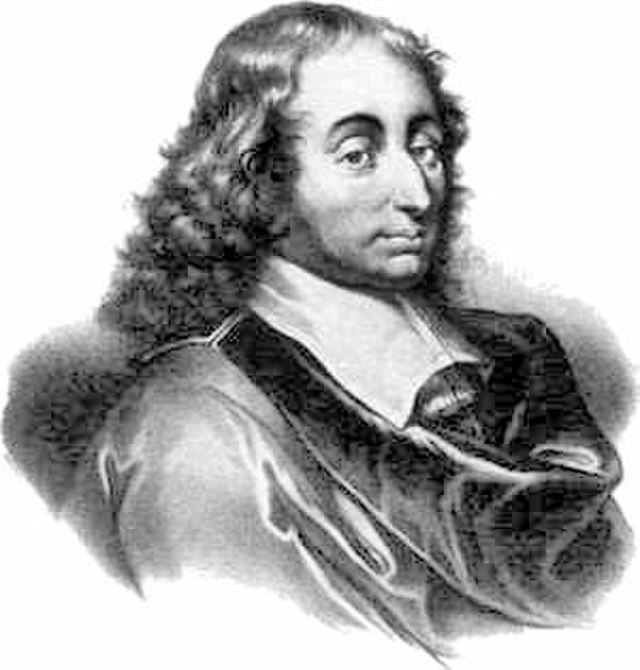
\includegraphics[scale=0.1]{images/persons/person_blaise_pascal.jpg}
                \caption{Blaise Pascal}
            \end{wrapfigure}

            However, those are purely mechanical and manual devices, main principle of which is very similar to how we convert numbers to different bases. They still
            require us to `translate' our numbers to abacus system and, after we've done our math, translate them back. \par
            
            The first succesful automation attempt is attributed to Blaise Pascal, with his \emph{Arithmetic Machine} which is also called a \emph{Pascaline}.
            It was designed and built between 1642 and 1644\footnote{\href{https://www.britannica.com/technology/Pascaline}{https://www.britannica.com/technology/Pascaline}}. 
            Pascaline could only add and subtract numbers, using rotational dials as an input.\par

            \begin{wrapfigure}{r}{0.6\textwidth}
                \centering
                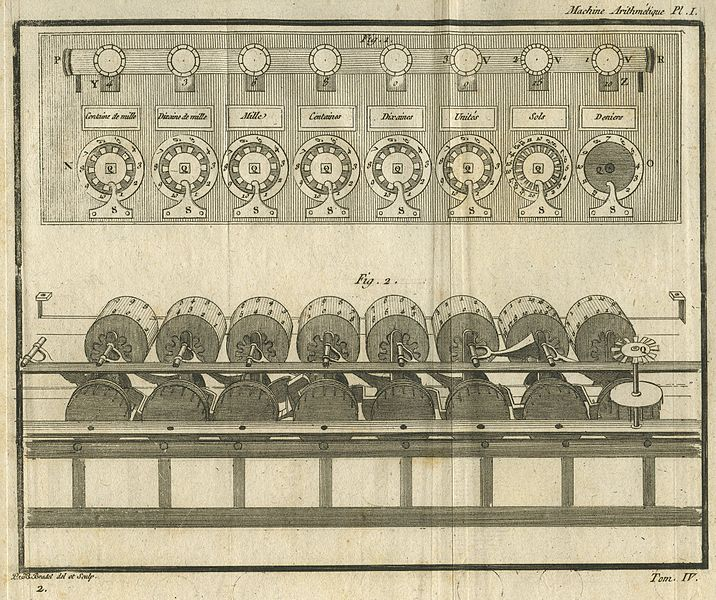
\includegraphics[scale=0.3]{images/devices/device_pascaline_scheme.jpg}
                \caption{Top view and overview of the mechanism}
            \end{wrapfigure}

            There are several pascalines still intact nowadays, most of the remaining ones are in european museums. Being the first calculator isn't the only achievement
            of pascaline. Pascal was only 18 years old, when he started designing his machine, trying to help his father with accounting. He went through about 50 prototypes
            before settled on the final one. Later Pascal presented his machine to the public, and, eventually, to the King of France, receiving a royal privilege, which 
            was basically a patent in those days. And yes --- his father did use it in work afterwards \par

            Pascaline wasn't a computer, but it was first in many ways --- first calculator, which was afterwards commercialized, used in business and patented. Many of 
            subsequent attemps to farther automate calculations were directly inspired by Pascaline. \par

            \begin{wrapfigure}{l}{0.3\textwidth}
                \centering
                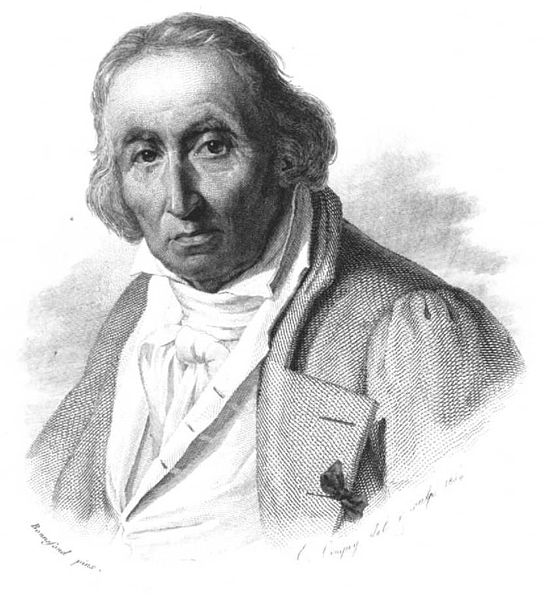
\includegraphics[scale=0.2]{images/persons/person_joseph_jacquard.jpg}
                \caption{Joseph Marie Jacquard}
            \end{wrapfigure}

            Next machine I want to discuss is not a computer either. It isn't even a calculator --- it's a loom. I cannot say much about weaving history, 
            but in computer history, it was indeed the most significant loom there is. In 1804 a french weaver and merchant, Joseph Marie Jacquard invented a \emph{Jacquard Machine}.

            Beginning of the 19\textsuperscript{th} century is pretty much a middle of industrial revolution. New fancy industrial looms are practically a 
            symbol of the new era. Industrial revolution changed our world forever, marking a \emph{transition from hand production methods to machines}.
            Despite Great Britain being the origin of the industrial revolution, it spread eventually over the continent, and afterwards, the world. 
            Industrial revolution eventually lead to the \emph{emergence of the capitalist economy}. In other words --- \emph{Industrial revolition was a big deal}. \par

            So, amidst all this revolution going, we could see how a work, that was being done by 100 men before can be done by 10 men with machines. It was \emph{super effecient}.
            Inventors tried to find a way to increase production effeciency (and therefore revenue) by exploring technical capabilities of the machines they worked with. So 
            Joseph Jacquard invented his machine, which was basically an \emph{attachment to the industrial loom}. A loom with an attached machine was subsequently called
            \emph{Jacquard Loom}\footnote{Jacquard Loom is a general term, which does not describe any concrete loom, but rather any loom with the control 
            mechanism, allowing pattern weaving automation}.

            \begin{wrapfigure}{r}{0.5\textwidth}
                \centering
                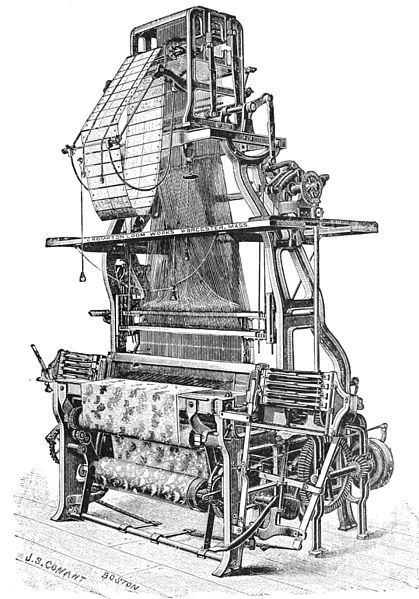
\includegraphics[scale=0.2]{images/devices/device_jacquard_loom.jpg}
                \caption{Jacquard Loom}
            \end{wrapfigure}

            The main purpose of Jacquard's attachment was an \emph{pattern weaving automation}. It used a chain of special cards laced together in a continuous, looped sequence.
            Those cards will later be called \emph{punch cards}. Punch card is, essentially a card, with designated spaces for holes. Later, some designated space would be `punched'
            to produce a hole in area. Some spaces were omitted during `punching'. After `punching' those holes we would have a card, partially filled with holes. Jacquard Loom
            relies on a simple mechanical action of those cards. While continuously moving, those cards would move controlling rods of the loom, therefore affect knot being weaved. 
            If there was no hole in the area, rod will move since card will push it. If there was a hole, rod wouldn't move since it would go through hole. \par

            \begin{wrapfigure}{l}{0.5\textwidth}
                \centering
                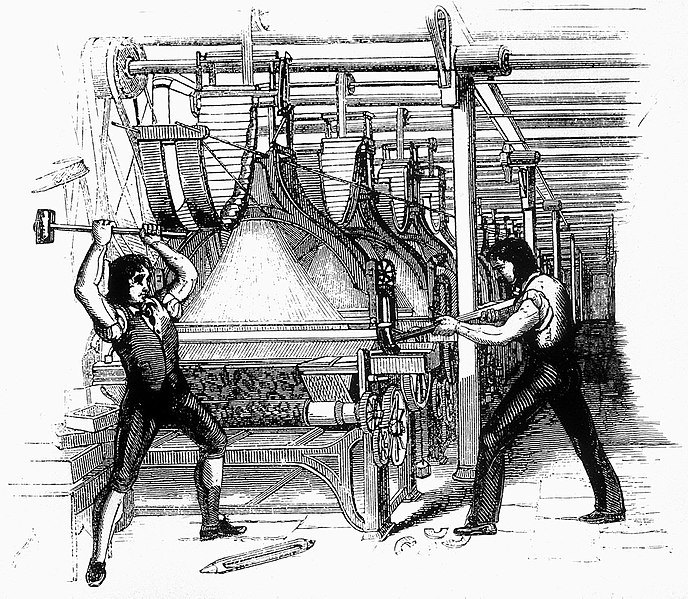
\includegraphics[scale=0.25]{images/misc/luddites.jpg}
                \caption{1844's depiction of Luddites destroying the loom}
            \end{wrapfigure}

            This machine would \emph{drastically} impact effeciency, since it was no longer required to be of high skill to weave complicate patterns. It, essentially, gave
            manufacturers ability to \emph{store design patterns and to reproduce them indefinitely}\footnote{At least until punch cards are in fine condition}. The man behind
            the punching process still needed to be trained and qualified, but to just reproduce a readily punched design wasn't much of an issue even to a low-skill worker.
            Just imagine a reaction from weavers, that used to work by hand. No surprise, that \emph{Luddites}\footnote{The term itself initially related to an organisation 
            of English textile workers. However, over time it has come to mean one opposed to new technologies in general}
            destroyed such machines to protest against their usage. \par

            Well, the idea of using automation in weaving patterns have touched deeply not only the Luddites, but also at least one mathematician, which was also a philosopher,
            inventor and mechanical engineer. It's just so happened this was also a man, who will be considered as the `father of the computer'\footnote{\href{https://cse.umn.edu/cbi/who-was-charles-babbage}
            {https://cse.umn.edu/cbi/who-was-charles-babbage}} by many. Some of his works even touched the subject of industrialization and economy, which influenced Karl 
            Marx\footnote{\href{https://projects.exeter.ac.uk/babbage/rosenb.html}{https://projects.exeter.ac.uk/babbage/rosenb.html}}. A man called Charles Babbage was deeply
            inspired by Joseph Jacquard's invention and intended to use his ingenious punch cards in his own machine. \par

            \begin{wrapfigure}{l}{0.3\textwidth}
                \centering
                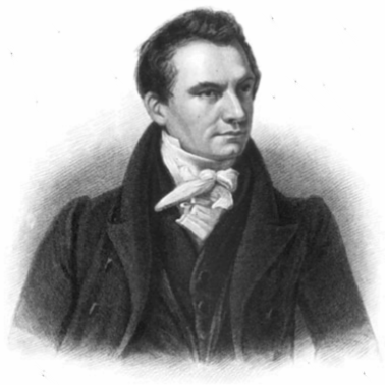
\includegraphics[scale=0.3]{images/persons/person_charles_babbage.png}
                \caption{Charles Babbage}
            \end{wrapfigure}

            Charles Babbage was an inventor of 2 machines, that are of interest in this essay: \emph{Difference Engine} and \emph{Analytical Engine}. Both of these machines
            were not finished in his lifetime, unfortunately. Nonetheless, this heritage of 2 unfinished machines marked a signinificant point in history of computers. More 
            than that, \emph{those 2 machines gave an opportunity for the first ever programmer to become a first ever programmer}. \par

            The Difference Engine, essentially was a giant mechanical calculator, that was powered by steam and printed results of it's computations in a table. 
            The format of the result was chosen due to being practical in that time --- many fields relied on tabular data to perform operations. One of the most
            notable example is a `Nautical Almanac', which was crucial for navigation and astronomy\footnote{\href{https://www.historyofinformation.com/detail.php?id=418}
            {https://www.historyofinformation.com/detail.php?id=418}}. But, constructing such a machine would require a formidable expenses and time. So, Babbage did what
            any startup nowadays would do --- he started seeking for investments. 
            In 1822, he wrote a letter\footnote{\href{https://play.google.com/books/reader?id=YBHnAAAAMAAJ&pg=GBS.PP2&printsec=frontcover&output=reader&hl=en}
            {https://play.google.com/books/reader?id=YBHnAAAAMAAJ\&pg=GBS.PP2\&printsec=frontcover\&output=reader\&hl=en}}
            to the President of Royal Society\footnote{Organization that exists to promote academic disciplines and science.}, in which he presented a 
            detailed explanation and description of his would-be machine\footnote{\href{https://www.historyofinformation.com/detail.php?id=450}
            {https://www.historyofinformation.com/detail.php?id=450}}. He also published this letter as pamphlet and sent it to other people, he deemed influential. \par

            One copy of this letter did reach a Lord of Treasury, who referred it to the Royal Society. After receiveing an endorsement letter and favorable report, Treasury
            decided to invest in Babbage's invention\footnote{\href{https://www.historyofinformation.com/detail.php?id=450}{https://www.historyofinformation.com/detail.php?id=450}}.
            Project ended up being at least 17 times more costly tnan initial estimate, not being finished at all, by the end of the next decade, eventually foundering in 1833. Babbage
            was initially granted a \textsterling1000, but for the next decade claimed a total sum of \textsterling17000 of goverment money. It can be roughly estimated to
            \textsterling2,150,000\footnote{\href{https://www.in2013dollars.com/uk/inflation/1833?amount=17000}{https://www.in2013dollars.com/uk/inflation/1833?amount=17000}}
            (around \$2,836,000) in 2022 money. \par

            In 1833 Charles Babbage threw a party, where he demostrated his guests, mostly members of high society, a part the Difference Engine. There were many
            guests that night, but we are interested in one in particular. One of the attendees was Lady Ada Byrone\footnote{She later will be known as Countess Ada Lovelace},
            the only legitimate child of Lord Baron, an English Poet. She showed an interest in this machine and became a life-long friend of Charles Babbage.
            Correspondence between the two is pretty well preserved to this day, providing insight to the next Babbage's invention. \par

            \begin{wrapfigure}{r}{0.5\textwidth}
                \centering
                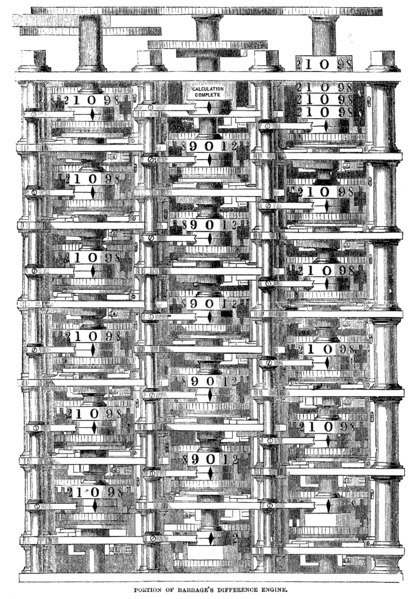
\includegraphics[scale=0.25]{images/devices/device_babbage_difference_engine.jpg}
                \caption{Part of Babbage's Difference Engine}
            \end{wrapfigure}

            As was mentioned before, Difference Engine project did end up exceeding given funding. Charles Babbage wasn't able to continue to work on his machine --- he couldn't
            afford his chief engineer in the project, Joseph Clement\footnote{Clement did end up owning all work he've done to himself, leaving Babbage virtually empty-handed}.
            This has lead Babbage to attempt an even more ambitious project in 1834 --- \emph{Analytical Engine}. While working on the Difference Engine, Babbage began to imagine
            ways of improving it, for it to support other kinds of calculations. Analytical Engine was something, we could call a computer in a general sense. It could be
            automated to perform any calculation set before it programmatically\footnote{\href{https://www.britannica.com/technology/Analytical-Engine}
            {https://www.britannica.com/technology/Analytical-Engine}}. However, this was purely on-paper project, we have no indications of any attempts to build it from Babbage. \par


            Analytical Engine was designed to consist of four major elements: the mill, the store, the reader and the printer. Functionally, modern computers pretty much
            repeat this architecture


            \begin{wrapfigure}{l}{0.3\textwidth}
                \centering
                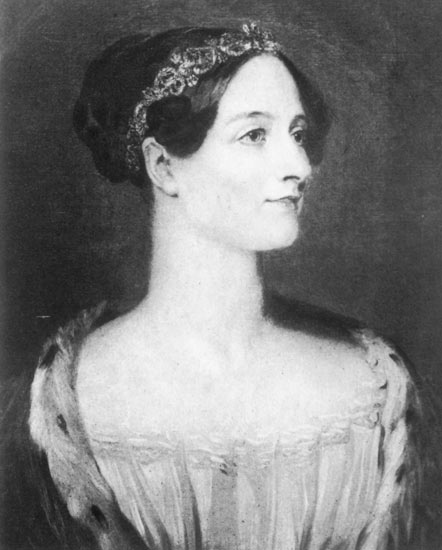
\includegraphics[scale=0.2]{images/persons/person_ada_lovelace.jpg}
                \caption{Augusta Ada King, Countess of Lovelace}
            \end{wrapfigure}

            \newpage
        \subsection{But can it speak?}
            \newpage


        

        %Pascal and Pascaline
        %Charles Babbidge
        %Ada Lovelace https://www.youtube.com/watch?v=IZptxisyVqQ
        %Jacquard Loom and punchcards https://www.youtube.com/watch?v=K6NgMNvK52A
        %Programming languages
        

    
\end{document}

